\documentclass{mcmthesis}
\mcmsetup{CTeX = false,
        tcn = 2514406, problem = B,
        sheet = true, titleinsheet = true, keywordsinsheet = true,
        titlepage = false, abstract = true}
\usepackage{palatino}
\usepackage{lipsum}
\usepackage{tocloft}
\usepackage{hyperref}
\usepackage{graphicx}
\usepackage{subcaption}
\usepackage{booktabs}
\usepackage{caption}
\usepackage{float}
\usepackage{enumitem}
\usepackage{amsmath}
\usepackage{algorithm}
\usepackage{algpseudocode}
\usepackage{xcolor}
\usepackage{colortbl}
\usepackage{wasysym}
\definecolor{tableheadercolor}{RGB}{255, 245, 205}
\captionsetup[table]{font=bf, labelfont=bf}

\renewcommand{\cftdotsep}{0.2}
\renewcommand{\cftsecpagefont}{\normalfont\hfill}
\renewcommand{\cftsecleader}{\cftdotfill{\cftdotsep}}
\renewcommand{\cftsecfont}{\bfseries}

\algnewcommand{\Switch}[1]{\State \textbf{switch} (#1) \algorithmicdo}
\algnewcommand{\Case}[1]{\State \hspace{1em} \textbf{case} #1:}
\algnewcommand{\Default}{\State \hspace{1em} \textbf{default}:}
\algnewcommand{\EndSwitch}{\algorithmicend \textbf{switch}}

\setlength{\cftsecindent}{0em}
\title{Revitalizing Tourism in a Sustainable Solution}

\setlength{\parindent}{0pt}

\begin{document}


\begin{abstract}
  {This study addresses sustainable tourism in Juneau, Alaska, USA, constructs a relevant model, and extends it to other over - toured areas.}

  {Juneau attracts many tourists, bringing income, but over-tourism causes problems. The Mendenhall Glacier is receding, reducing tourists, income, and experience. It also pressures local infrastructure, and local residents are dissatisfied due to housing and living issues.}

  {For Objectives 1 and 2, a multi-objective optimization model for sustainable tourism is built. With economic, environmental, and social goals at its core and tourist numbers and percentages as decision variables, it aims to maximize economic income, minimize per-unit carbon emissions, and ease infrastructure pressure. Constraints like tourist limits are set, and a genetic algorithm screens impact weights. Results show rational tourist number control can cut carbon footprint and infrastructure pressure while growing tourism revenue.}

  {An additional revenue-expenditure plan allocates revenue to environmental protection, infrastructure, etc. A sensitivity analysis of the model is done.}

  {For Objectives 3 and 4, the model is extended to Harbin. Due to differences in environment and extreme - weather - amplified infrastructure pressure, the model is adjusted for Harbin's special constraints. Visitor promotion is modeled, with a recommendation index for less-visited areas.}

  {For Objective 5, a memo for Juneau's tourist council proposes balancing tourism by limiting visitors, adjusting funding, and developing new attractions. Extra revenues should support the environment, infrastructure, and community.}

  {This study offers scientific policy support for Juneau and a case for other over-toured areas, and its adaptable and multi-objective model is a key reference for sustainable tourism development.}
  \begin{keywords}
    Sustainable Tourism; Invisible Burden; Genetic Algorithm
  \end{keywords}
\end{abstract}

\maketitle
\tableofcontents
\newpage

\section{Introduction}
\subsection{Problem Background}
% Problem Background:简单来说,就是对赛题进行补充说明。
% 例如题目是关于新能源汽车的问题,题目中没有提到电池续航,所以可以查相关文献,用自己的话复述下文献里的一些语句即可。
% 建议:写完论文正文部分之后,再根据正文里的内容来写背景,但注意不要在这部分提到任何模型或解题思路,也不要照搬比赛题目中的内容。
{In Juneau, Alaska, tourism is a large part of the city's economy. While it generates a great deal of revenue for the city, over-tourism also creates several problems.}

{First, the percentage of residents who believe that tourism development has had a large impact on their lives has continued to rise over the past period (2002, 2006, 2021, 2022, 2023) as Figure \ref{fig:Figure1} shows.\cite{1}}

\begin{figure}[h]
  \small
  \centering
  \includegraphics[width=15cm]{Comparison Overall Impact of Tourism on Households, 2002, 2006, 2021, 2022, 2023.pdf}
  \caption{\textbf{Comparison Overall Impact of Tourism on Households}} \label{fig:Figure1}
\end{figure}

{The Mendenhall Glacier is one of Juneau's most important attractions and attracts many tourists yearly. \textbf{However}, Mendenhall Glacier has been melting since the last century and has become even faster in recent years under the influence of Juneau's over-tourism development. Since 2007, the glacier has retreated the equivalent of eight soccer fields. The Figure \ref{fig:Figure2} below show how the Mendenhall Glacier will change from 1984 to 2023.\cite{2}\cite{3}}

\begin{figure}[htbp]
  \centering
  \begin{subfigure}[b]{0.49\textwidth}
      \includegraphics[width=\textwidth]{mendenhallglacier1984.jpg}
      \caption{August 17, 1984}
      \label{fig:first_image}
  \end{subfigure}
  \hfill
  \begin{subfigure}[b]{0.49\textwidth}
      \includegraphics[width=\textwidth]{mendenhallglacier2023.jpg}
      \caption{July 28, 2023}
      \label{fig:second_image}
  \end{subfigure}
  \caption{\textbf{Comparison: area of Mendenhall Glacier in 1984 and 2023}}
  \label{fig:Figure2}
\end{figure}

{In addition to the melting of the glaciers, other specific impacts include increased congestion in the city center due to the arrival of tourists, and whale-watching boats and their wake have also significantly impeded normal traffic. The percentage of residents who feel that their lives have been affected to a greater or greater extent has increased over the past five years.}

{Therefore,how to mitigate the above problems while maintaining stable tourism revenues and at the same time lowering the carbon footprint and reducing pollution to the environment is a pressing issue for Juneau today.}

\subsection{Restatement of the Problem}
% Restatement of the Problem: 用自己的话,把赛题每一小问的关键语句重述一遍。该部分内容不要写的过多,专有名词不要更换:
% Considering the background information and restricted conditions identified in the prob-lem statement, we need to solve the following problems:
% Problem 1
% Problem 2
% Problem 3
{Juneau, Alaska is a famous tourist city with mythical landscape. Through in-depth analysis and research of the background of the problem, combined with specific constraints, the objectives can be restated as follows:}
\begin{itemize}
  \item \textbf{Objective 1: }Develop a sustainable tourism model for Juneau that takes into account factors such as the number of visitors, total revenue, and measures put in place to stabilize the tourism industry.
  \item \textbf{Objective 2: }Develop an additional revenue plan to promote sustainable tourism.
  \item \textbf{Objective 3: }Apply the model we have developed to other over-tourism areas by adjusting for some special factors.
  \item \textbf{Objective 4: }Use our model to promote locations with fewer visitors to achieve a better balance.
  \item \textbf{Objective 5: }Compose a memorandum to the tourist council of Juneau. This  memorandum was to include our projections, the impacts of the various measures, and our recommendations on how to optimise the results.
\end{itemize}


%%\subsection{Literature Review}
% Literature Review:文献综述就是把关于当前问题的现有研究成果做个概述。首先需要阅读大量解决该问题的论文,其次得用自己的话总结出来。
% 除非想冲O奖,否则别写这部分。一来竞赛时间有限,不可能去阅读大量论文;二来能力有限,不一定能写好总结。 
% 小技巧:去搜相关论文,一般发表的论文都会有文献综述部分,照着别人的综述用自己的话描述一遍即可。
%%{here is the literature review}


\subsection{Related Reports and Status}
\begin{figure}[H]
  \small
  \centering
  \includegraphics[width=7cm]{What is your preference for future cruise passenger volume in Juneau.pdf}
  \caption{\textbf{What is your preference for future cruise passenger volume in Juneau?}} \label{fig:Figure3}
\end{figure}
{The CBJ (City and Borough of Juneau) has now done something to address these issues. In terms of the overall management of tourism, more than half of the respondents felt that they were not doing enough, which is considerably higher than in previous years. Their specific measures have focused on limiting the number of cruise ships, for example to five large ships per day, but still half of the respondents would like to see even fewer ships as Figure \ref{fig:Figure3} shows.}


{On top of that, CBJ has to deal with multiple invisible burden, as shown in Figure \ref{fig:Figure4}.\cite{4}}

\begin{figure}[h]
  \small
  \centering
  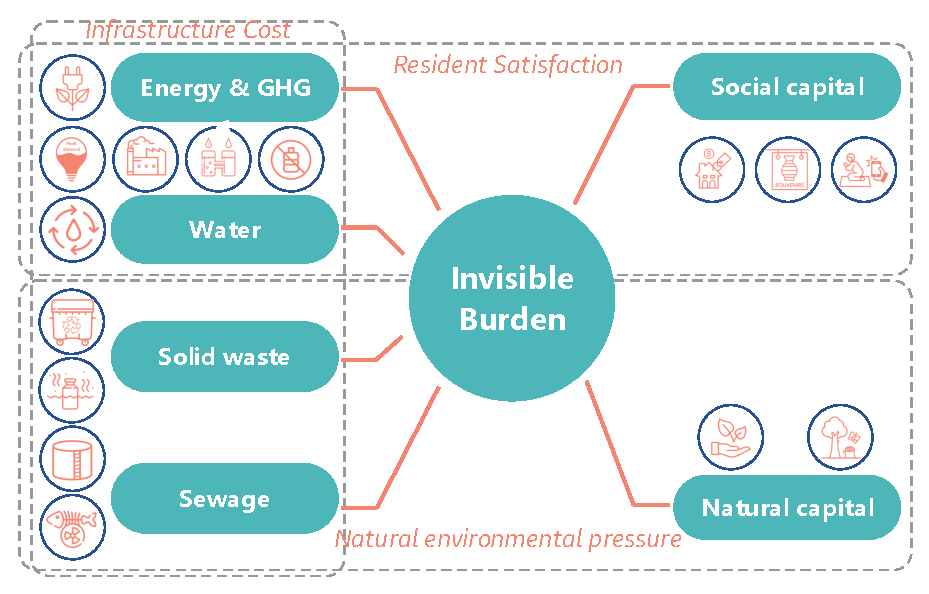
\includegraphics[width=\textwidth]{Invisible Burden.eps}
  \caption{\textbf{Invisible Burden}} \label{fig:Figure4}
\end{figure}

{Taken together with the context of the problem, the hidden costs to the local area of increased tourist numbers can be broadly categorized into three areas:}
\begin{itemize}
  \item \textbf{Pressure on natural environment} 
  \item \textbf{Pressure on infrastructure} 
  \item \textbf{Residents' satisfaction} 
\end{itemize}


{It can be seen that the measures currently taken by the CBJ have not been well received and that they are inherently more limited and less accepted among the respondents. Therefore,they need a more balanced and integrated approach to the development of sustainable tourism.}

\subsection{Overview of Our Work}
% Our Work:这个小部分主要介绍论文的分析思路和建模的框架,
% 有点像国赛论文中的问题分析部分,可以画个思维导图(可用软件亿图图示),大家可以学习。
{Based on the comprehensive review of the existing reports and surveys, our work mainly includes the following:}

\Huge\textbullet
\normalsize{\textbf{Model I :Sustainable Tourism Model for Objective 1 and Objective 2}}
\begin{itemize}
  \item {Four influence factor models to consider the different influences generated by tourists}
  \item {Sustainable tourism model that combines different factors}
  \item {Enhanced sustainable tourism model considering addition revenue andexpenditure}
  \item {A set of plan for expenditures from additional revenue}
\end{itemize}
\Huge\textbullet
\normalsize{\textbf{Model II :Attraction Promotion Model for Objective 3 and Objective 4}}
\begin{itemize}
  \item {Adaption of the model to another tourist destination impacted by overtourism}
  \item {Recommand model for promoting locations with fewer visitors to achieve a better balance.}
\end{itemize}
\Huge\textbullet
\normalsize{\textbf{A one-page Memo to tourist council of Juneau for Objective 5}}

{In summary, the whole modeling process can be shown in the following Figure \ref{fig:Figure5}.}

\begin{figure}[H]
  \small
  \centering
  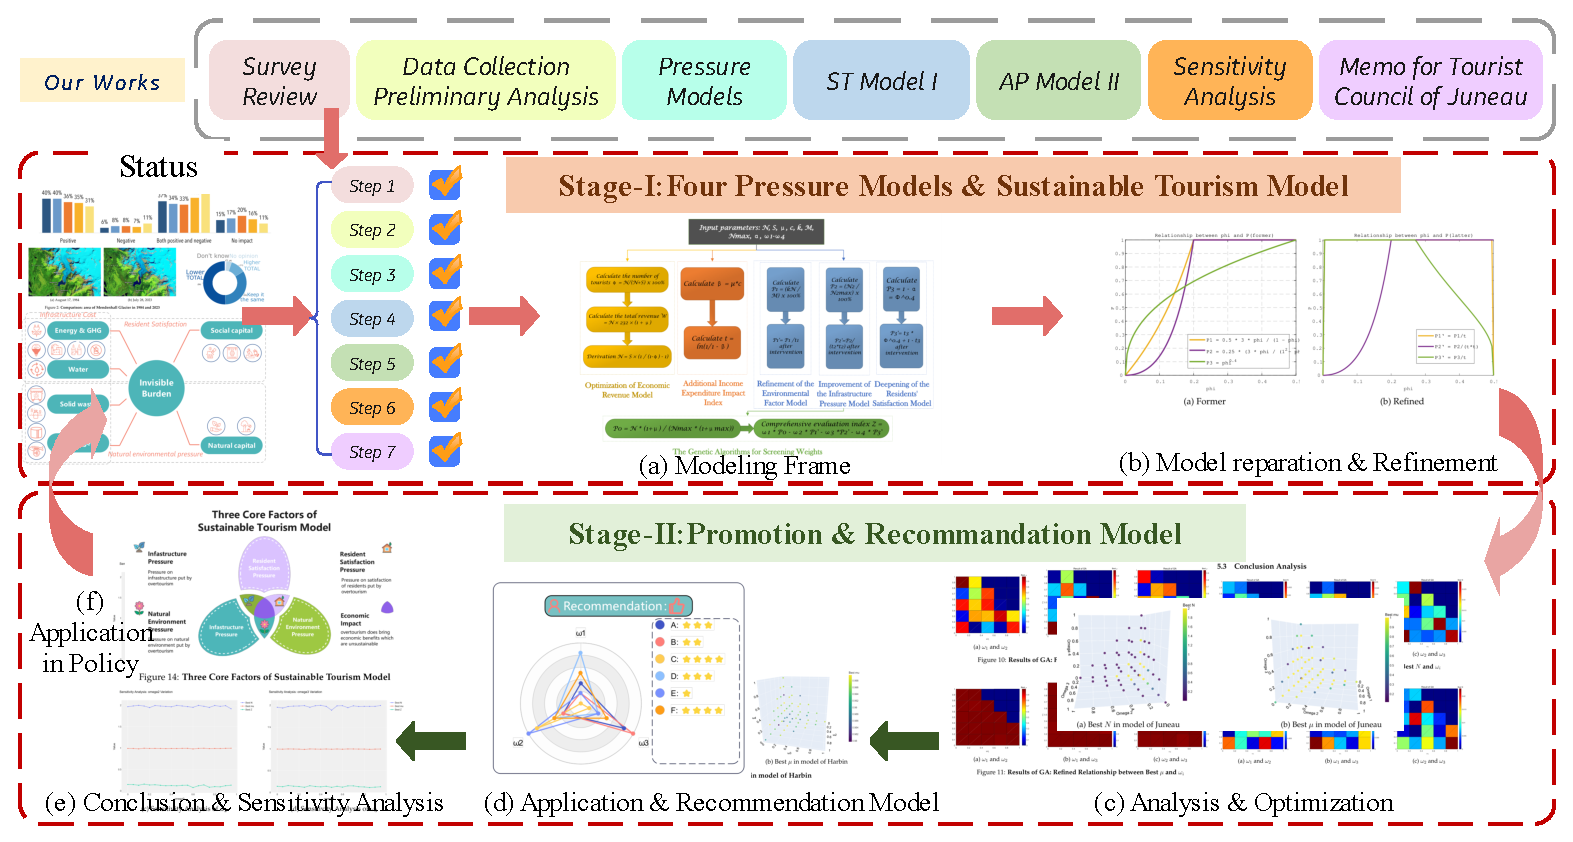
\includegraphics[width=\textwidth]{Our Work.eps}
  \caption{\textbf{Our Work}} \label{fig:Figure5}
\end{figure}

\section{Assumptions and Justifications}
% Justification翻译过来是正当理由的意思。这一部分要写模型假设,并且要对论证假设的合理性,
%这一点比国赛的要求要高,请大家引起足够的注意。
{Considering the practical situation contains various complex factors, this paper makes reasonable assumptions to simplify the problems. And each hypothesis is closely followed by its corresponding justifications:}
\begin{itemize}
  \item \textbf{Assumption 1: Tourists traveling to the same attraction have roughly the same level of consumption, which can be measured by the level of consumption per capita.}
  
  $\Rightarrow$ \textbf{Justification:} The same attraction is more distinctive and attracts visitors with similar interest preferences, even if the visitors come from different regions and classes.
  \item \textbf{Assumption 2: The number of residents in tourist destinations remains constant and is not affected by changes in the number of tourists.}
  
  $\Rightarrow$ \textbf{Justification:} The natural growth and migration of residents of tourist destinations are more stable than those of mobile groups of tourists. The number of inhabitants of tourist destinations does not change drastically in a short period of time.
  \item \textbf{Assumption 3: The taxes collected are considered to be borne entirely by the tourists.}
  
  $\Rightarrow$ \textbf{Justification:} In addressing the problem of overtourism, the ultimate bearer of the tax increase is the tourist community.
  \item \textbf{Assumption 4: The carbon footprint capacity of tourist destination attractions remains constant throughout the year.}
  
  $\Rightarrow$ \textbf{Justification:} In a healthy and stable ecosystem, the ecological niches of individual species are relatively stable, and environmental regulation does not change significantly. Ecosystem stability is an important prerequisite for sustainable tourism.
  \item \textbf{Assumption 5: Measures to limit the number of tourists and measures to increase taxes are independent of each other, and changes in tax rates do not change tourists' willingness to travel.}
  
  $\Rightarrow$ \textbf{Justification:} Over-tourism destinations are already attractive enough to attract excess tourists, and even an increase in the tax rate would have minimal effect on tourists' willingness to travel.
  \item \textbf{Assumption 6: No global public health event or disasters.}
  
  $\Rightarrow$ \textbf{Justification:} Considering the impact of COVID-19 on the global tourism industry in 2020, such similar large-scale events are difficult to predict. We assumed that there would be no future events that would be destructive to the tourism industry.
\end{itemize}


\section{Notations and Description}
% Notations是对模型中使用的重要变量进行说明,表格形式三线表,
% 表头分别是Symbol(符号)、Description(含义)、Unit(单位)(可不写),一般排版时尽量放到一页中。
% 注意:
% 只需写主要模型用到的重点变量、全篇通用的变量
% 求解计算等过程中的局部变量不要写
% 符号要以公式的形式写;如果是物理量,可在描述里写单位
% 每个符号的描述要简短,控制在一行内
{The key mathematical notations used in this paper are listed in the following Table \ref{tab:notations}. Some variables are not listed here and will be introduced once we use them.}
\begin{table}[H]
    \centering
    \caption{\textbf{Notations used in our paper}}\label{tab:notations}
    \begin{tabular}{cc}
        \toprule
        \textbf{Symbol} & \textbf{Description} \\
        \midrule
        $P_1$ & Pressure indicator of natural environment that tourists put $(0,1)$  \\
        $P_2$ & Pressure indicator of infrastructure that tourists put $(0,1)$  \\
        $P_3$ & Pressure indicator of resident satisfaction that tourists put $(0,1)$ \\
        $\mu$ & Tax rate $(0,1)$ \\
        $N$ & Number of tourists (described by 10,000 persons) \\
        $S$ & Number of residents (described by 10,000 persons) \\
        $\alpha$ & Residents' satisfaction $(0,1)$ \\
        $\varphi$ & Tourist proportion $(0,1)$ \\
        $M$ & Maximum total carbon footprint of tourists that the environment can carry \\
        $W$ & Total revenue (described by dollars) \\
        $X$ & Basic consumption of tourists (described by dollars) \\
        $k$ & Carbon footprint per tourist \\
        $t$ & Additional income expenditure impact index \\
        $\omega_i$ & Weight of the $i$-th influence factor (i=0,1,2,3)\\
        \bottomrule
    \end{tabular}
\end{table}


\section{Model Preparation}
\subsection{Data Collection}
{Since this problem does not directly provide relevant data, finding available data became one of the most critical challenges.Through the pre-requirement analysis of the mathematical model, we needed to gather related information about the tourism of Juneau, such as the geographical characteristics, surveys of Juneau passengers, and the residents' feelings about tourism, etc.}

{The official website of City and Borough of Juneau was queried, and various data in the aspect of tourism and ecology were obtained. Furthermore, the main data resources including data websites and related references are shown in the following Table \ref{tab:data_source_collation}.}

\begin{table}[H]
  \centering
  \caption{Data source collation}\label{tab:data_source_collation}
  \begin{tabular}{ccc}
  \toprule
  \textbf{Data Description} & \textbf{Data Resources} & \textbf{Types} \\
  \midrule
  Area Features & https://earthobservatory.nasa.gov/ & Geography \\
  Related information & https://juneau.org/ & Policy \\
  Icefield of Juneau& https://explore.openaire.eu/ & Ecology \\
  Juneau Travel Data & https://www.maasaimara.com/ & Economy \\
  Surveys & https://www.alaskatia.org/resources/research/ & Economy \\
  Map and Image & https://www.mapbox.com/ & Image \\
  Other Datasets & https://datasetssearch.research.google.com/ & Mixed \\
  \bottomrule
  \end{tabular}
  \label{tab:data_source_collation}
\end{table}
\subsection{Preliminary Analysis}
{Before considering the details of the model, we preclarified the general idea of the model, presented in Figure \ref{fig:Figure6}.}
\begin{figure}[H]
  \small
  \centering
  \includegraphics[width=\textwidth]{Modeling Mind Map.pdf}
  \caption{\textbf{Modeling Mind Map}} \label{fig:Figure6}
\end{figure}

\section{Model I :Sustainable Tourism Model}
\subsection{Model Construnction and Analysis}
{Considering the Objective presented above,
this paper translates the effects caused by tourists into the sustainable
tourism model.}

\subsubsection{Optimization of Economic Revenue Model}
{Assuming the total revenue as $W$, the tax rate
as $\mu$, the number of tourists as $N$, and the number of residents as $S$, with each tourist's basic
consumption set at a constant of $X = 232$ dollars(data from 2023). In this cenario, the formula for
calculating total revenue $W$ is:}
\begin{equation}
  W=N\times X\times(1+\mu)
\end{equation}

{Furthermore, we define the tourist proportion $\varphi$
as the ratio of the number of tourists to the total population (i.e., the sum
of tourists and residents), mathematically expressed as:}
\begin{equation}
  \varphi = \frac{N}{N+S} \times 100 \%
\end{equation}

{From this, we can derive the relationship
between the number of tourists $N$, the number of
residents $S$, and the tourist proportion $\varphi$:}
\begin{equation}
  N = S\times\big [\frac{1}{(1 - \varphi)} - 1) \big ]
\end{equation}
{Taking the 2023 data as an example, if the
number of tourists $N$ is $2$ and the number of residents S is $3$ (data from 2023,described by 10,000 persons), then
the tourist proportion $\varphi$ is $40\%$.}

\subsubsection{Refinement of the Environmental Factor Model}
{To assess the limitation of environmental
factors on tourist capacity, we set the per capita carbon footprint of tourists as $k$ and the
maximum tourist carbon footprint that the environment can carry as $M$. Then, the
capacity constraint $P_1$ of environmental factors on tourists can be expressed
as:}
\begin{equation}
  P_1=\frac{kN}{M}\times 100\%
\end{equation}

{Assuming that in 2023, when the maximum daily
number of tourists $N_{max}=2$,(data from 2023,described by 10,000 persons) $P_1=1$, substituting and solving yields:
}
\begin{equation}
  P_1=0.5N
\end{equation}

{Taking into account the Additional Income Expenditure Impact Index $t$. Increased funding for nature conservation should theoretically increase the environment's carrying capacity, i.e., the maximum amount of the total carbon footprint generated by tourists that the environment can carry, thus affecting  $P_1$.} 

{Defining $t$ as:}
\begin{equation}
  t = \ln\left(\frac{1}{1 - \mu}\right)
  \end{equation}

{We can further refine the environmental factor model as:}
\begin{equation}
  P_1'=P_1\times\frac{1}{t}=\frac{kN}{Mt}\label{eq:p1}
\end{equation}

{This model takes into account the additional income expenditure impact index $t$ and the effect of increased funding on the environment's carrying capacity. The model is a refinement of the original model, which only considers the effect of the environmental factors on tourist capacity.}

{In subsequent revisions, we will continually use $t$ to characterize the impact of additional revenue expenditures.}
\subsubsection{Improvement of the Infrastructure Pressure Model}
{Infrastructure pressure $P_2$ has a quadratic
relationship with the number of tourists and there exists a maximum reasonable
capacity $N_{max}$. Therefore, we set the following relationship:}
\begin{equation}
  P_2=\frac{N^2}{N_{max}^2}\times 100\%
\end{equation}
{Similarly, assuming that in 2023, when the
maximum daily number of tourists Nmax=20,000, P2=1, substituting and solving
yields:}
\begin{equation}
  P_2=0.25 N^2
\end{equation}

{Increased funding for infrastructure improvements will increase $N_{max}$, thus affecting $P_2$ for the same number of tourists. Taking $t$ into account, we can further refine the infrastructure pressure model as:}
\begin{equation}
  P_2'=P_2\times\frac{1}{t^2}=\frac{N^2}{N_{max}^2t^2}\label{eq:p2}
\end{equation}
{This model reveals how infrastructure pressure
rises sharply with the increase in tourist numbers, providing important
decision-making basis for managers.}
\subsubsection{Deepening of the Residents' Satisfaction Model}
{Residents' satisfaction $\alpha$ is a key indicator
for measuring residents' attitudes towards the impact of tourism. We set the
proportion of residents with a positive attitude towards the impact of
tourism at $31\%$, serving as the initial value of
satisfaction. The dissatisfaction level $P_3$ of residents towards the increase in
tourists can be measured by $1-\alpha$. Through power function fitting, we obtain
the following relationship:}
\begin{equation}
  P_3=1-\alpha=\varphi^\lambda =\left(\frac{N}{N+S}\right)^\lambda
\end{equation}
{Substituting $\varphi =40\%$ and $\alpha =31\%$(data from 2023) into the equation,
we solve for $\lambda =0.4$. Therefore, the
residents' satisfaction model can be expressed
as:}
\begin{equation}
  P_3=1-\alpha=\left(\frac{N}{N+S}\right)^{0.4}
\end{equation}

{Increased funding to enhance resident satisfaction may increase $\alpha$ by improving residents' living conditions, providing compensation, etc., thus affecting $P_3$. And $P_3=1-\alpha$ , so after intervention:}
\begin{equation}
  P_3'=1-\alpha \times t=t \times \varphi ^{0.4}+1-t
\end{equation}
{For ease of calculation, it is approximated that:}
\begin{equation}
P_3'=\frac{P_3}{t}=\frac{1}{t}\left(\frac{N}{N+S}\right)^\lambda\label{eq:p3}
\end{equation}
{This model takes into account the effect of increased funding on residents' satisfaction. The model is a refinement of the original model, which only considers the effect of the residents' satisfaction on tourist capacity.}

{Above all, we limit the range of $P1$, $P2$, and $P3$ to $[0,1]$, and refine the model by taking into account the additional income expenditure impact index $t$. The comparisons are shown in Figure \ref{fig:Figure7} below.}
\begin{figure}[htbp]
  \centering
  \begin{subfigure}[b]{0.49\textwidth}
      \includegraphics[width=\textwidth]{Relationship between phi and P Former.eps}
      \caption{Former}
      \label{fig:former}
  \end{subfigure}
  \hfill
  \begin{subfigure}[b]{0.49\textwidth}
      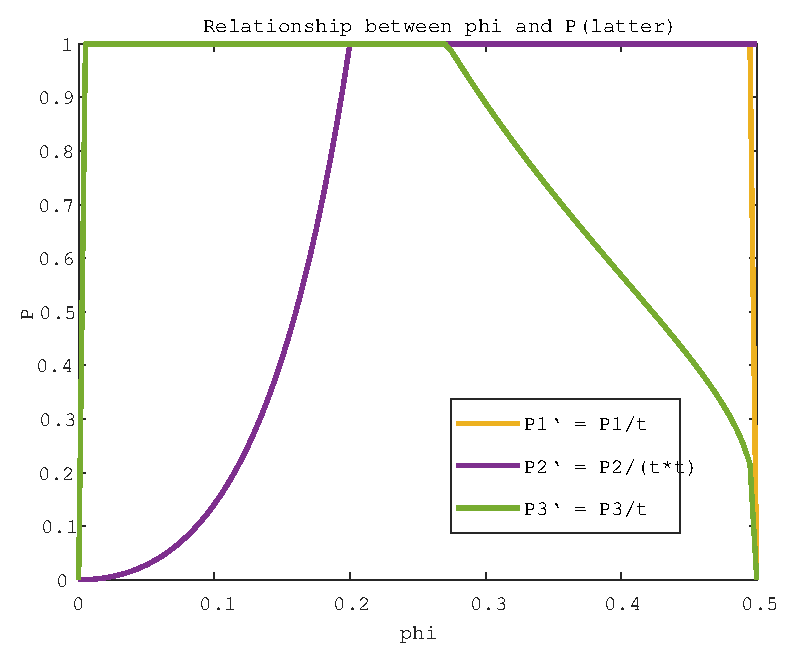
\includegraphics[width=\textwidth]{Relationship between phi and P Refined.eps}
      \caption{Refined}
      \label{fig:latter}
  \end{subfigure}
  \caption{\textbf{Relationship between phi and P}}
  \label{fig:Figure7}
\end{figure}

\subsection{Comprehensive Evaluation}

{Let the comprehensive evaluation index be $Z$, and the weight coefficients be $\omega _0$, $\omega _1$, $\omega _2$, and $\omega _3$, respectively. Then:}
\begin{gather}
  Z=\omega_0 P_0-\omega_1 P_1'-\omega_2 P_2'-\omega_3 P_3'\\
  P_0=\frac{N (1+\mu)}{Nmax (1+\mu_{max})}\label{eq:p0}
\end{gather}
{In this formula, $N_{max}$ represents the maximum number of tourists, and  $\mu_{max}$ represents the maximum tax rate.
Due to the complex constraints involving multiple variables in this model, it falls into the category of nonlinear programming problems, prompting the selection of the genetic algorithm for solution. The genetic algorithm is an optimization algorithm that mimics natural selection and genetic mechanisms. It searches for optimal solutions in the solution space by simulating selection, crossover, and mutation operations in the biological evolution process. This algorithm is suitable for dealing with complex multivariate nonlinear optimization problems and can quickly find approximate optimal solutions in a large solution space.}

{For Juneau, the parameters of the function \eqref{eq:p1} \eqref{eq:p2} \eqref{eq:p3} \eqref{eq:p0} are set as follows:}
\begin{equation}
  \begin{cases}
  Z=\omega_0 P_0-\omega_1 P_1'-\omega_2 P_2'-\omega_3 P_3'\\
  P_1'=\frac{0.5N}{t} \\
  P_2'=\frac{0.25N^2}{t^2} \\
  P_3'=\frac{1}{t}\left(\frac{N}{N+3}\right)^{0.4} \\
  P_0=\frac{N (1+\mu)}{2 (1+\mu_{max})} \\
  t = \ln\left(\frac{1}{1 - \mu}\right) \\
  \omega_i \in [0,1], \ i = 0,1,2,3 \\
  \sum\limits_{i=0}^3 \omega_i = 1 \\
  \end{cases}
  \end{equation}


\begin{itemize}
  \item \textbf{Encoding: }{The decision variables $N$ (number of tourists) and $\mu$ (adjustment ratio of tourism-related taxes and fees) are encoded to enable them to be processed by the genetic algorithm, forming chromosomes in the context of the genetic algorithm.}
  \item \textbf{Initial Population Generation: }{A certain number of individuals are randomly generated to form the initial population. The encoding of each individual is randomly generated within the value range to ensure population diversity and avoid the algorithm getting stuck in local optimal solutions.}
  \item \textbf{Fitness Function: }{The objective function $Z$ is taken as the fitness function. For each individual in the population, the values of $N$ and $\mu$ are obtained by decoding their encoding, and these values are substituted into the objective function to calculate the fitness value. A higher fitness value indicates that the individual performs better in achieving sustainable tourism development goals and has a greater probability of being selected in the selection process of the genetic algorithm.\cite{5}\cite{6}}
\end{itemize}
{In the actual problem, different weights $\omega_1$, $\omega_2$, $\omega_3$ reflect the weight of the three factors regarded by the local government, that is degree of emphasis. The difference in the relationship between the optimal tax rate and the number of tourists under different degrees of emphasis provides a theoretical basis for alleviating the over-tourism pressure on tourist places while harmonizing the economic benefits.}
\subsection{Conclusion Analysis}
\begin{figure}[H]
  \centering
  \begin{subfigure}[b]{0.3\textwidth}
      \includegraphics[width=\textwidth]{omega_1&2_best_n_form.eps}
      \caption{$\omega_1$ and $\omega_2$}
      \label{fig:12Nf}
  \end{subfigure}
  \hfill
  \begin{subfigure}[b]{0.3\textwidth}
      \includegraphics[width=\textwidth]{omega_1&3_best_n_form.eps}
      \caption{$\omega_1$ and $\omega_3$}
      \label{fig:13Nf}
  \end{subfigure}
  \hfill
  \begin{subfigure}[b]{0.3\textwidth}
      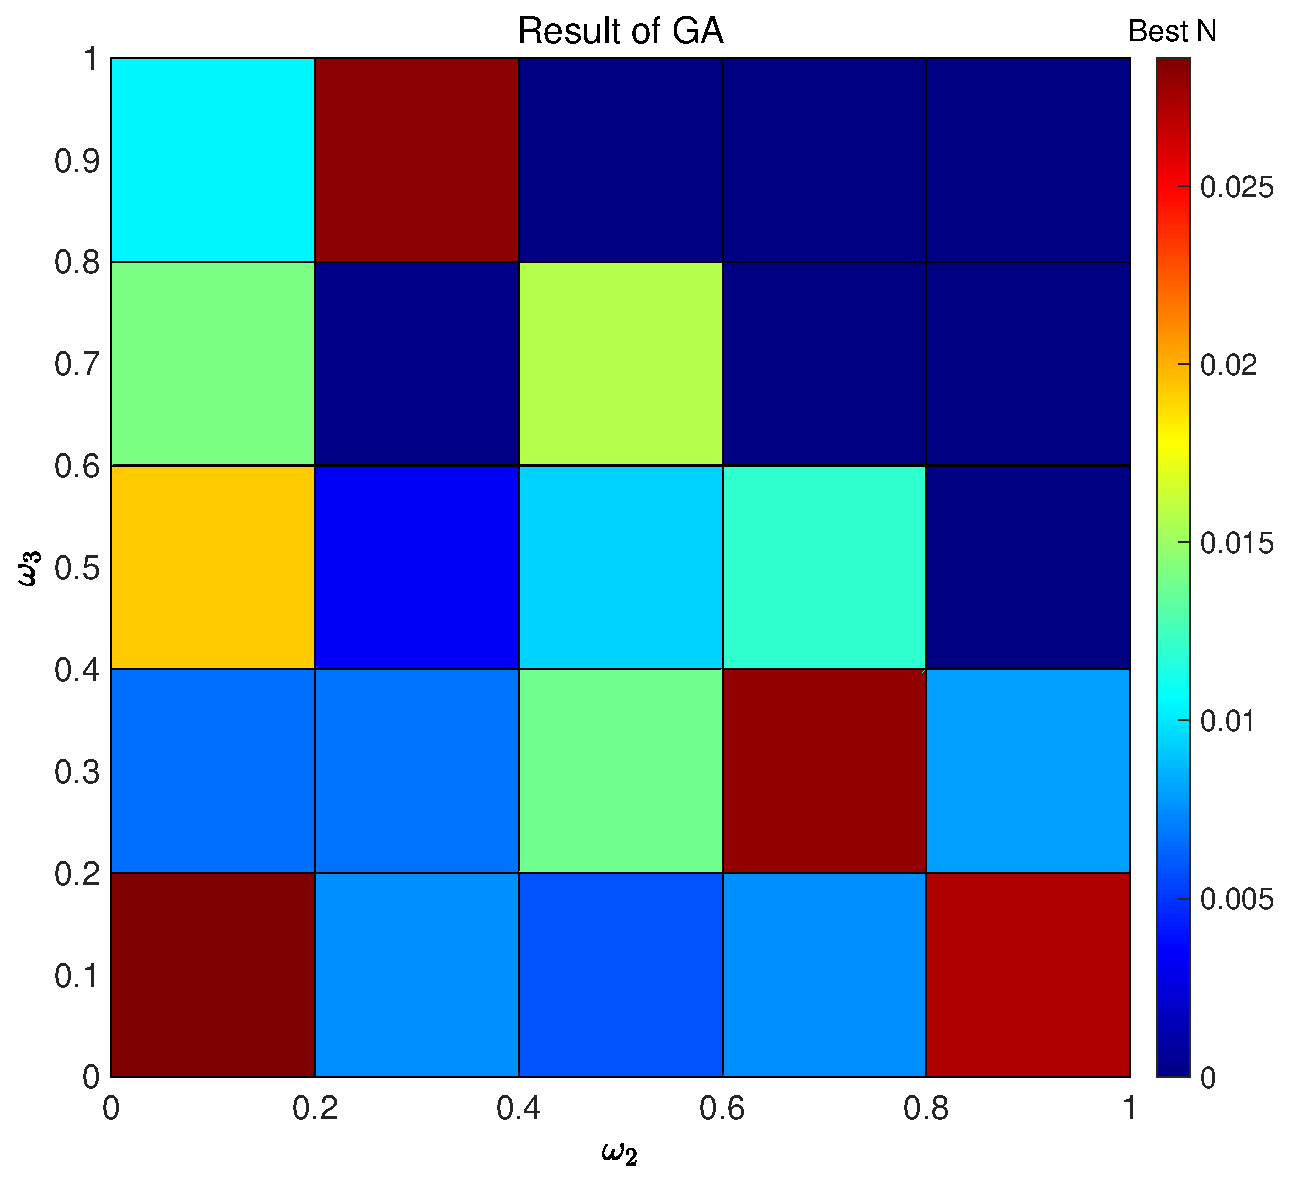
\includegraphics[width=\textwidth]{omega_2&3_best_n_form.eps}
      \caption{$\omega_2$ and $\omega_3$}
      \label{fig:23Nf}
  \end{subfigure}
  \caption{\textbf{Results of GA: Former Relationship between Best $N$ and $\omega_i$}}
  \label{fig:Figure8}
\end{figure}

\begin{figure}[H]
  \centering
  \begin{subfigure}[b]{0.3\textwidth}
      \includegraphics[width=\textwidth]{omega_1&2_best_n_post.eps}
      \caption{$\omega_1$ and $\omega_2$}
      \label{fig:12Np}
  \end{subfigure}
  \hfill
  \begin{subfigure}[b]{0.3\textwidth}
      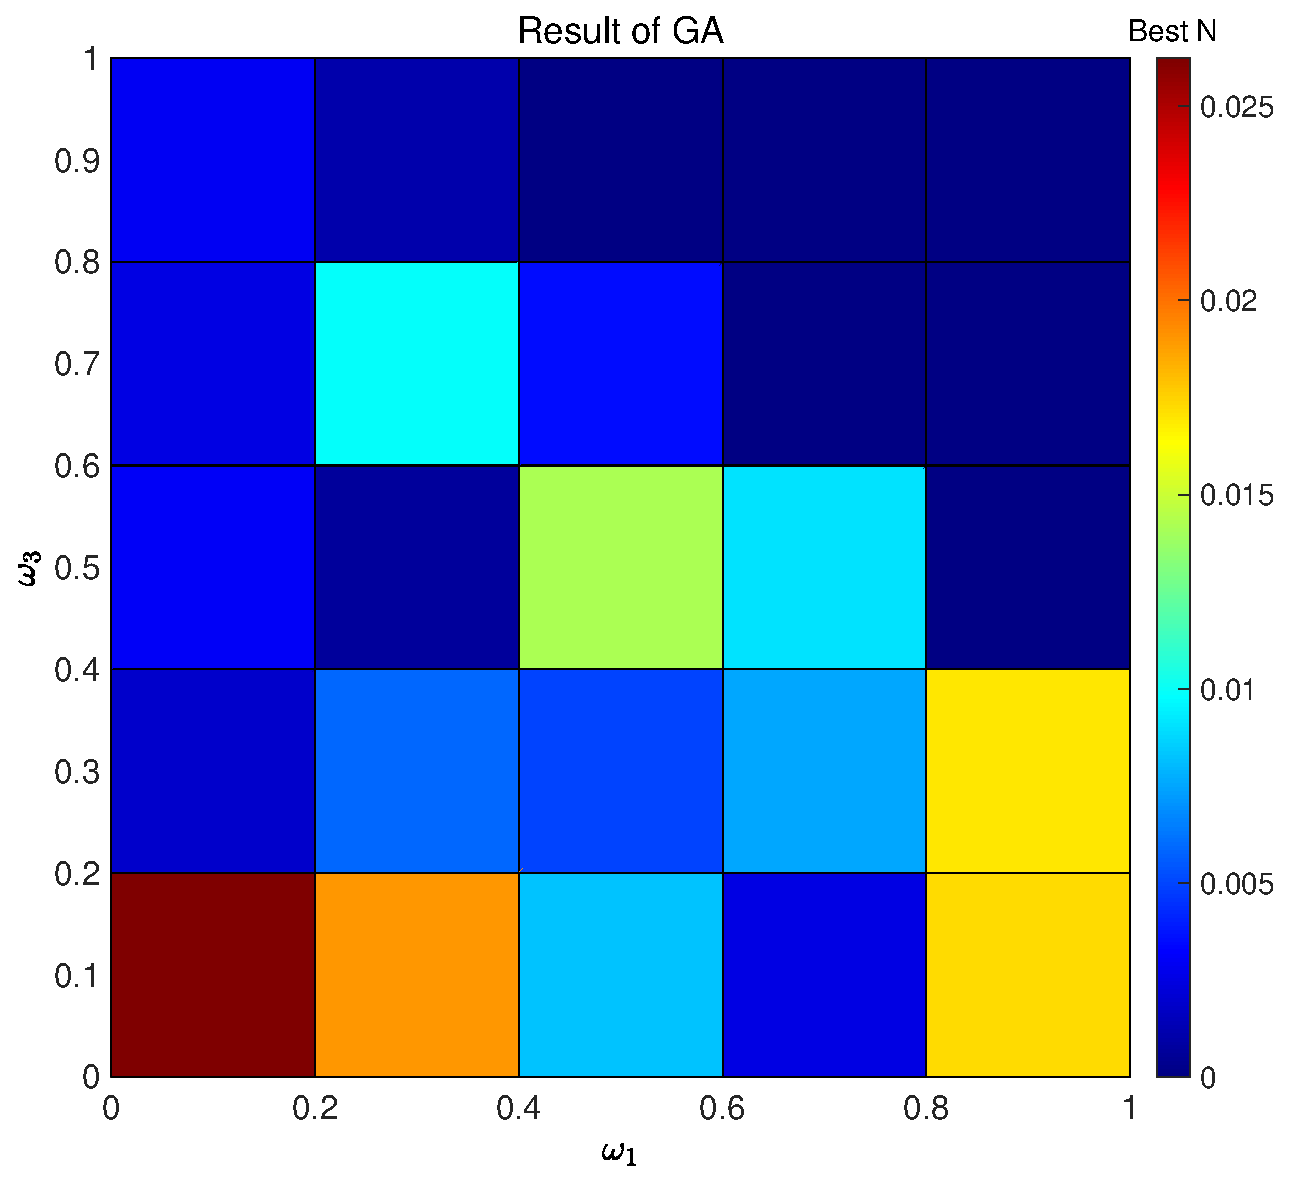
\includegraphics[width=\textwidth]{omega_1&3_best_n_post.eps}
      \caption{$\omega_1$ and $\omega_3$}
      \label{fig:13Np}
  \end{subfigure}
  \hfill
  \begin{subfigure}[b]{0.3\textwidth}
      \includegraphics[width=\textwidth]{omega_2&3_best_n_post.eps}
      \caption{$\omega_2$ and $\omega_3$}
      \label{fig:23Np}
  \end{subfigure}
  \caption{\textbf{Results of GA: Refined Relationship between Best $N$ and $\omega_i$}}
  \label{fig:Figure9}
\end{figure}

\begin{figure}[H]
  \centering
  \begin{subfigure}[b]{0.3\textwidth}
      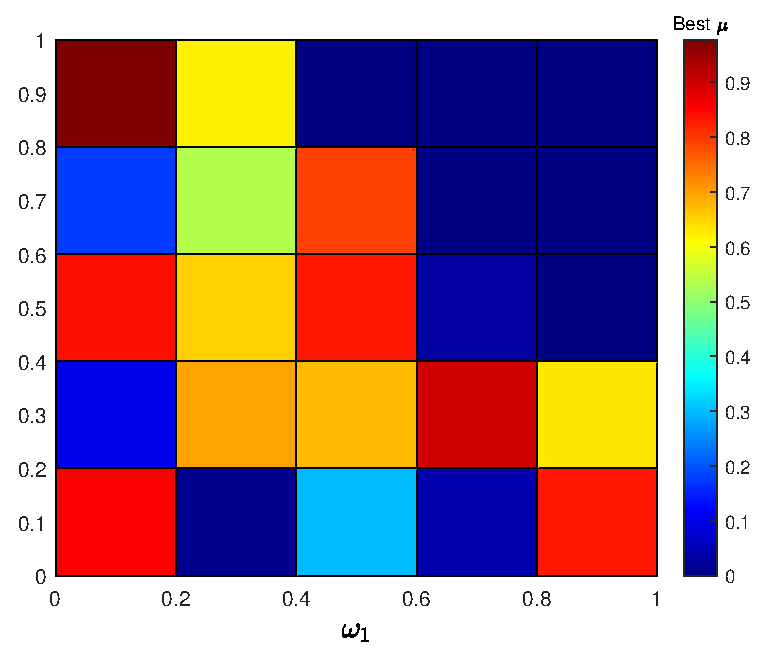
\includegraphics[width=\textwidth]{omege_1&2_best_mu_form.eps}
      \caption{$\omega_1$ and $\omega_2$}
      \label{fig:12muf}
  \end{subfigure}
  \hfill
  \begin{subfigure}[b]{0.3\textwidth}
      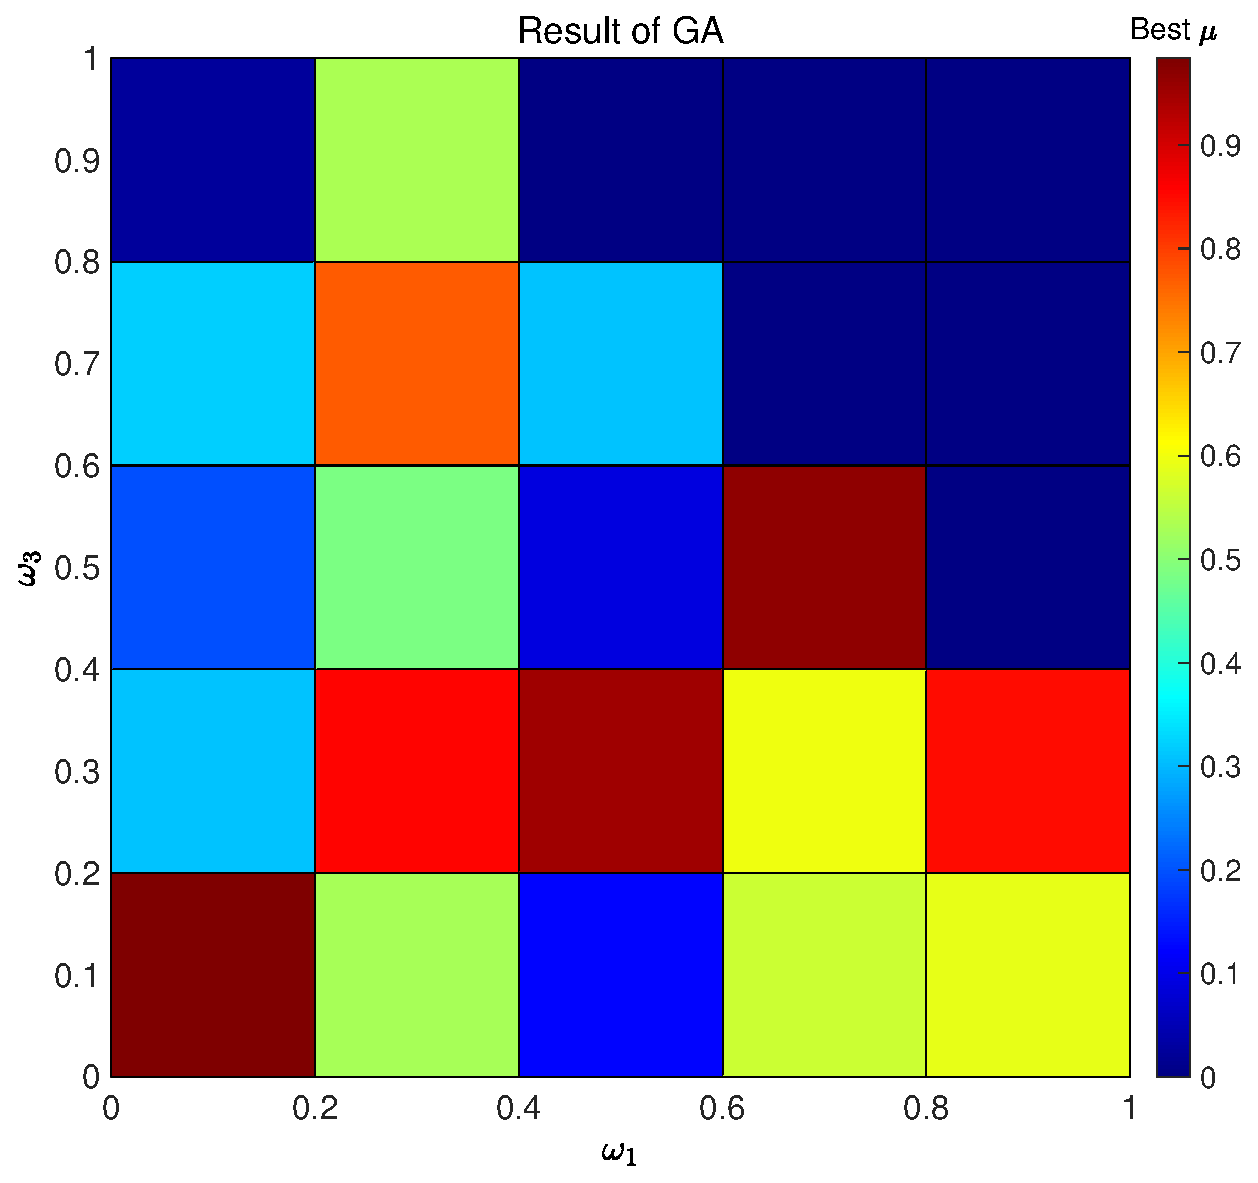
\includegraphics[width=\textwidth]{omega_1&3_best_mu_form.eps}
      \caption{$\omega_1$ and $\omega_3$}
      \label{fig:13muf}
  \end{subfigure}
  \hfill
  \begin{subfigure}[b]{0.3\textwidth}
      \includegraphics[width=\textwidth]{omega_2&3_best_mu_form.eps}
      \caption{$\omega_2$ and $\omega_3$}
      \label{fig:23muf}
  \end{subfigure}
  \caption{\textbf{Results of GA: Former Relationship between Best $\mu$ and $\omega_i$}}
  \label{fig:Figure10}
\end{figure}

\begin{figure}[H]
  \centering
  \begin{subfigure}[b]{0.3\textwidth}
      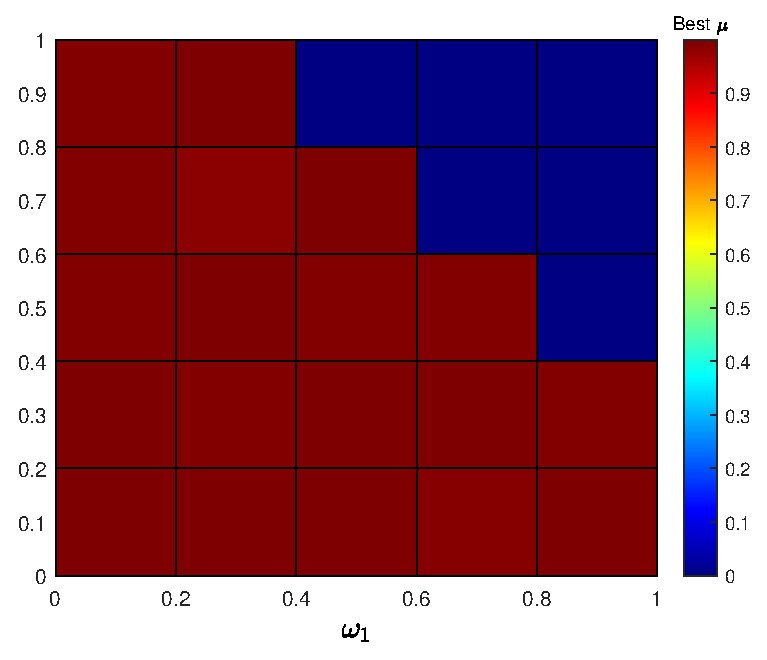
\includegraphics[width=\textwidth]{omege_1&2_best_mu_post.eps}
      \caption{$\omega_1$ and $\omega_2$}
      \label{fig:12mup}
  \end{subfigure}
  \hfill
  \begin{subfigure}[b]{0.3\textwidth}
      \includegraphics[width=\textwidth]{omega_1&3_best_mu_post.eps}
      \caption{$\omega_1$ and $\omega_3$}
      \label{fig:13mup}
  \end{subfigure}
  \hfill
  \begin{subfigure}[b]{0.3\textwidth}
      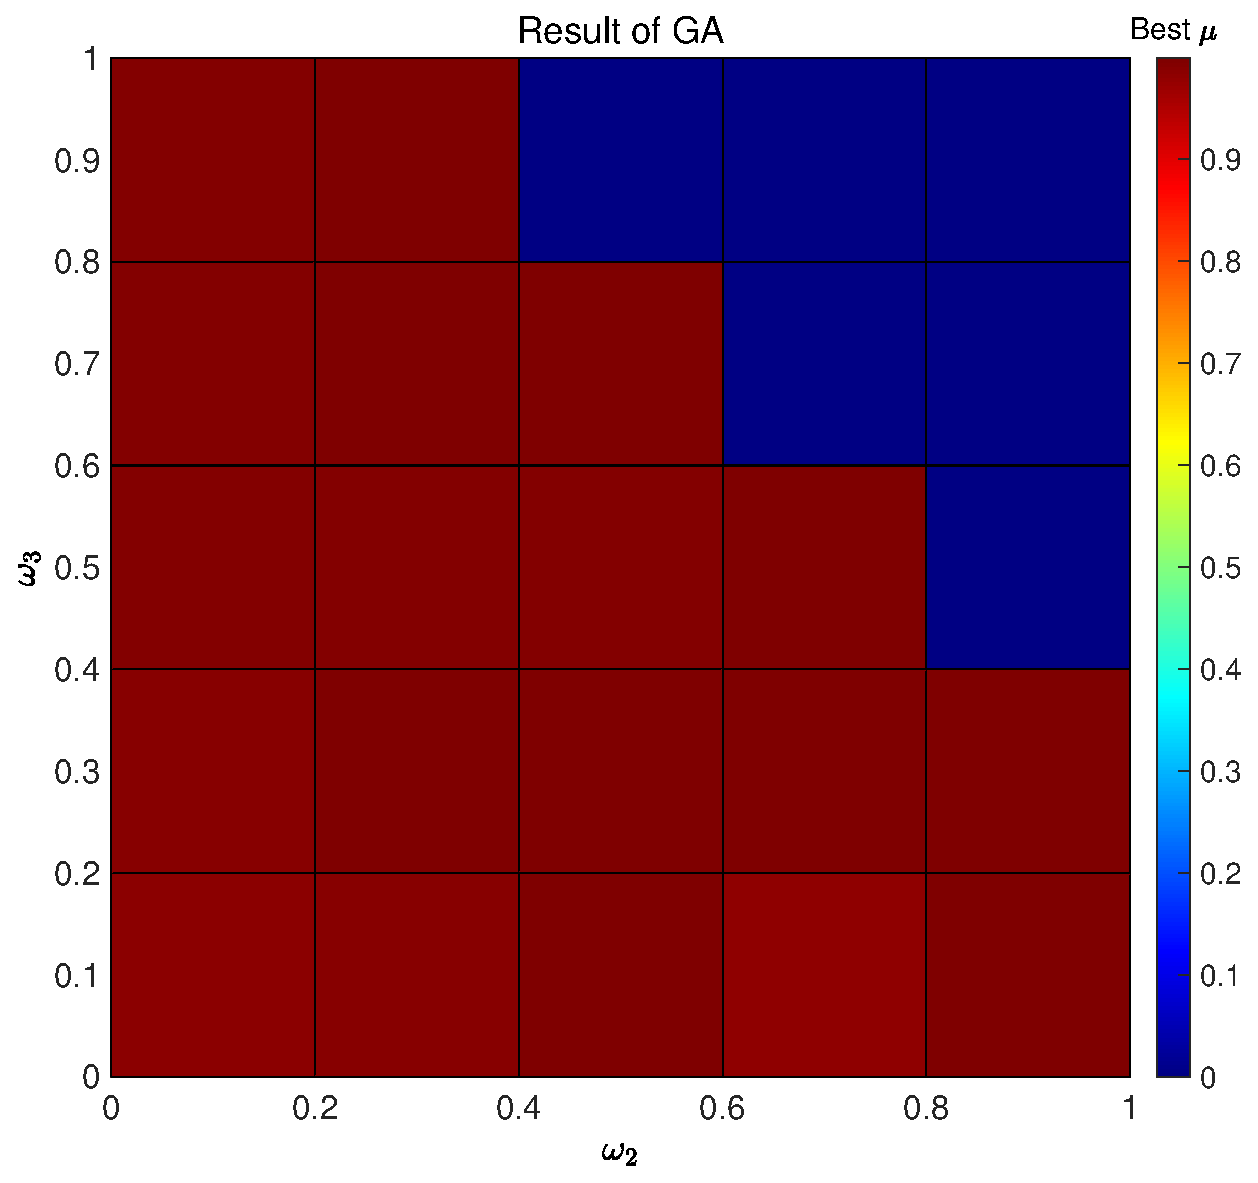
\includegraphics[width=\textwidth]{omega_2&3_best_mu_post.eps}
      \caption{$\omega_2$ and $\omega_3$}
      \label{fig:23mup}
  \end{subfigure}
  \caption{\textbf{Results of GA: Refined Relationship between Best $\mu$ and $\omega_i$}}
  \label{fig:Figure11}
\end{figure}

{These two set of figures (Figure \ref{fig:Figure9} and Figure \ref{fig:Figure11}) show the optimal $M$ and $\mu$ values for different weights of the other two factors, controlling for the weight of one of the factors. When a tourist destination makes decisions, it can find the optimal number of tourists and tax rate in the corresponding checkerboard-like graph by taking different weights depending on the importance given. In Figure \ref{fig:Figure8} and Figure \ref{fig:Figure10}, the previous image is only used as a comparison to prove the necessity of optimization.}

\begin{figure}[H]
  \centering
  \begin{subfigure}[b]{0.4\textwidth}
      \includegraphics[width=\textwidth]{juneau_best_n_1.png}
      \caption{Best $N$ in model of Juneau}
      \label{JNn}
  \end{subfigure}
  \hfill
  \begin{subfigure}[b]{0.4\textwidth}
      \includegraphics[width=\textwidth]{juneau_best_mu_2.png}
      \caption{Best $\mu$ in model of Juneau}
      \label{JNmu}
  \end{subfigure}
  \caption{\textbf{GA Result: Best $N$ and $\mu$ in model of Juneau}}
  \label{fig:JNnmu}
\end{figure}

{As policymakers place more emphasis on environmental protection, infrastructure development, and resident satisfaction, the amount of money spent on these items in the optimal decision will increase, and the maximum number of tourists per day in the constraints will decrease, which is consistent with our common sense and corroborates the validity of our model.}

{Based on the results of Figure \ref{fig:JNnmu}, the following advice is given:}
\begin{itemize}
  \item \textbf{Adivce 1: Juneau should appropriately limit the number of daily tourists so that Juneau's tourism industry has better sustainability.}
  
  {After limiting the number of tourists per day, $N$ decreases, resulting in high $Z$ values. In the case of higher $\omega_1$, $\omega_2$, and $\omega_3$, i.e., policy decisions that emphasize environmental pressures, infrastructural pressures, and resident satisfaction pressures, $N$ is limited to the optimal amount, which increases the Z-value achieving the goal of sustainable tourism.}
  \item \textbf{Adivce 2: Juneau should appropriately increase the taxes collected so that Juneau's tourism industry is more sustainable.}
  
  {Increasing the tax rate $\mu$ will decrease $Z$ values, which indicates that the tourism industry is more sustainable. However, the optimal tax rate should be determined based on the economic situation of Juneau. Therefore, the optimal tax rate should be determined based on the economic situation.}
\end{itemize}
{In conclusion, we confirm the validity of measures such as limiting the number of tourists and collecting taxes, which are now underway in the city of Juneau, and that the intensity of these measures should be adjusted in real time over the next few years to ensure the sustainability of Juneau's tourism industry, based on yearly tourism data and the emphasis placed on different factors by the local government.}
\section{Model II :Attraction Promotion Model}
\subsection{Model Applications in Other Destinations}
{For the completed sustainable tourism model, different destinations essentially only change the maximum number of tourists for each pressure in the model, and by adjusting the parameters in the existing formula, a comprehensive assessment of other destinations under different weights can be obtained. The following is an example of a tourist destination, Harbin, also from three areas, to demonstrate the portability of the model.}

\begin{itemize}
  \item \textbf{Pressure on natural environment:} {Harbin is famous for its ice and snow, which attracts a large number of tourists. Compared to the glacier in Juneau, Harbin's environment is less affected by the pressure of tourists' carbon footprints and can accommodate more tourists' carbon footprints, and $M$ should be larger(set $N_{max}=122$, data from 2024,described by 10,000 persons).}
  \item \textbf{Pressure on infrastructure:} {Considering the impact of extreme weather amplifies to some extent the effect of pressure generated by tourists on the maintenance of infrastructure, resulting in a relative reduction in tourist capacity (using the number of residents 8,000,000 of 2024 as a reference).}
  \item \textbf{Residents' satisfaction:} {In terms of local residents' satisfaction, based on the same assumptions, the relationship between $P_3$ and $\alpha$ is considered to be the same as in the current model.}
\end{itemize}
{Based on the above considerations, the sustainable tourism model as follows of Harbin is obtained after making adjustments to the parameters of the existing model:}
\begin{equation}
  \begin{cases}
  Z=\omega_0 P_0-\omega_1 P_1'-\omega_2 P_2'-\omega_3 P_3'\\
  P_1'=\frac{0.3N}{t} \\
  P_2'=\frac{0.4N^2}{t^2} \\
  P_3'=\frac{1}{t}\left(\frac{N}{N+800}\right)^{0.4} \\
  P_0=\frac{N (1+\mu)}{122 (1+\mu_{max})} \\
  t = \ln\left(\frac{1}{1 - \mu}\right) \\
  \omega_i \in [0,1], \ i = 0,1,2,3 \\
  \sum\limits_{i=0}^3 \omega_i = 1 \\
  \end{cases}
  \end{equation}

{The results are obtained by genetic algorithm processing:}

\begin{figure}[H]
  \centering
  \begin{subfigure}[b]{0.4\textwidth}
      \includegraphics[width=\textwidth]{harbin_best_n_2.png}
      \caption{Best $N$ in model of Harbin}
      \label{HRBn}
  \end{subfigure}
  \hfill
  \begin{subfigure}[b]{0.4\textwidth}
      \includegraphics[width=\textwidth]{harbin_best_mu_2.png}
      \caption{Best $\mu$ in model of Harbin}
      \label{HRBmu}
  \end{subfigure}
  \caption{\textbf{GA Result: Best $N$ and $\mu$ in model of Harbin}}
  \label{fig:HRB}
\end{figure}

{It can be seen that under different weights, different results are obtained based on the number of tourists and tourism tax in Harbin as well. From this different emphasis on the policy can give the corresponding number of tourists and tax rate program.}

{From this, we realize the application of the sustainable tourism model in other regions by taking Harbin as an example.Also, We drew an introductory diagram describing the main three areas when applying the model to other destinations as Figure \ref{fig:Problem Deconstruction} shows.}

\begin{figure}[H]
  \small
  \centering
  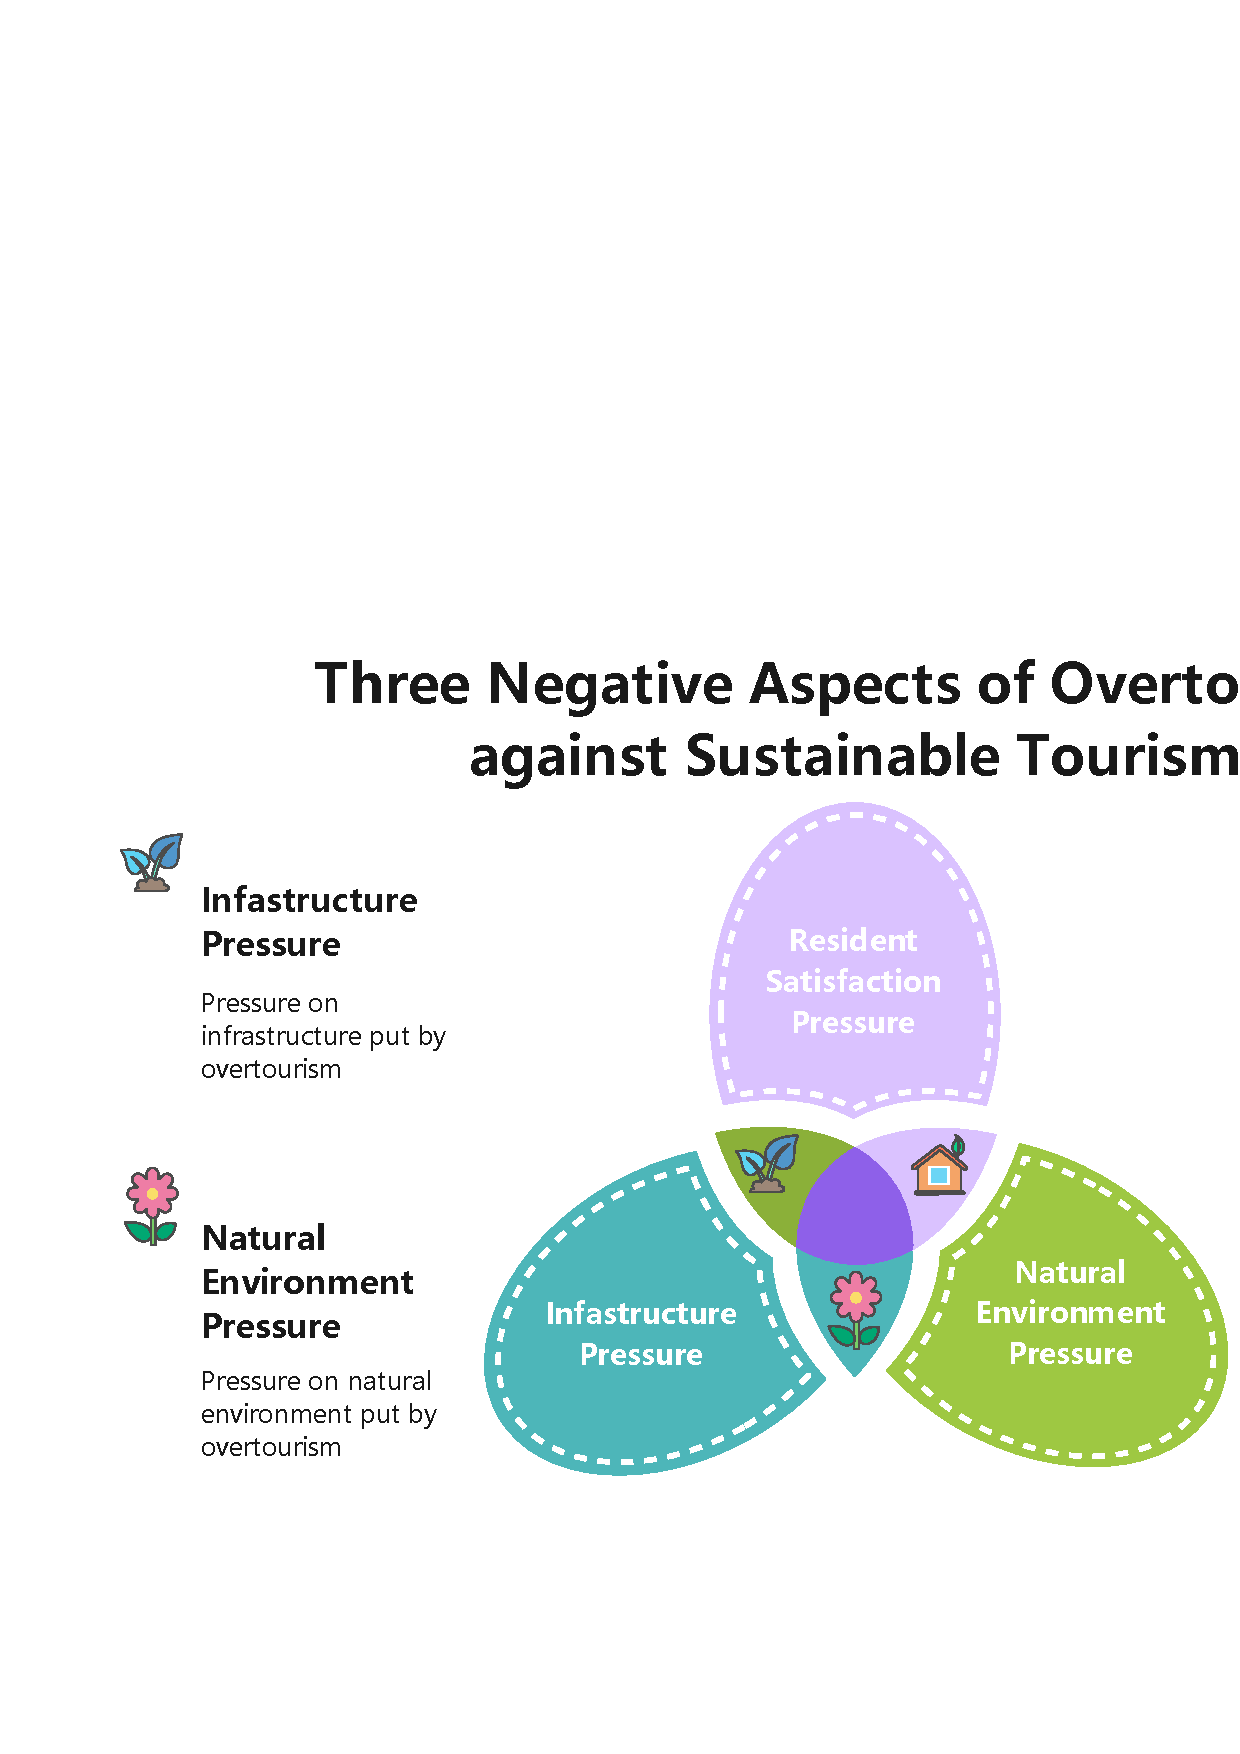
\includegraphics[width=12cm]{Problem Deconstruction.png}
  \caption{\textbf{Three Core Factors of Sustainable Tourism Model}} \label{fig:Problem Deconstruction}
\end{figure}

\subsection{Visitor Recommendation Model}
{Based on the sustainable tourism model developed above, we developed a tourist attraction scoring model for tourists, i.e., a tourist promotion model. The aim is to give tourists a recommendation of different attractions in terms of their current impact on the number of tourists and to guide tourists to tend to shift their destinations to attractions with a lower number of tourists.}

{For intuitive reasons, we plan to create a recommendation index from 1 to 5 stars, which should combine the impacts of the number of tourists on the environmental capacity, infrastructure, and residents' satisfaction, as well as the different levels of importance that the local government attaches to these impacts. As can be seen from the existing model section, we can combine the weights and pressure indices for the given weights and pressure indices into a composite indicator by using the following formula:}
{$\frac{\sum\limits_{i=1}^3 \omega_i P_i}{\sum\limits_{i=1}^3 \omega_i}$}
{Then, the definition domain is transformed into a five-star rating, in which more stars indicate a higher recommendation, and combined with the previous model to obtain a visitor promotion model:}
  \begin{equation}
    R = 5\cdot(1-\frac{\sum\limits_{i=1}^3 \omega_i P_i}{\sum\limits_{i=1}^3 \omega_i})
    \quad\text{in which} \quad
    \begin{cases}
    P_1'=\frac{kN}{Mt} \\
    P_2'=\frac{N^2}{N_{max}^2t^2} \\
    P_3'=\frac{1}{t}\left(\frac{N}{N+S}\right)^\lambda \\
    t = \ln\left(\frac{1}{1 - \mu}\right) 
    \end{cases}
  \end{equation}
{$R$ is defined as the recommendation index. Based on mathematical definitions above, we have designed a Python program for our
visitor recommendation models as follows:}

\begin{algorithm}[H]
  \caption{Visitor Recommendation Model for Given Destination}
  \begin{algorithmic}[1]
      \State \textbf{Input}: $k, M, \mu, \lambda, N_{max}, N, S$
      \State \textbf{Output}: $R, \omega_1, \omega_2, \omega_3$
      \State Initialize the desired variables based on $k, M, \mu, \lambda, N_{max}, N, S$;
      \For{$\omega_i = 0$ \textbf{to} $1$ $(i=1,2,3)$}
          \State According to $k, M, \mu, \lambda, N_{max}, N, S$, calculate the corresponding values of $P_1', P_2', P_3'$;
          \State Calculate $Z$ based on different weights and pressure indices;
          \State Do genetic algorithm to find the optimal values of $N$ and $\mu$;
      \EndFor
      \State Select optimal values of $\omega_1, \omega_2, \omega_3$;
      \State Calculate $R$ based on the optimal values of $\omega_1, \omega_2, \omega_3$;
      % \Procedure{Switch}{$R$}
      \Switch{$R$}
          \Case{$R \leq 1$}
              \State $R \gets 1$
          \Case{$1 < R \leq 2$}
              \State $\vdots$
          \Case{$R > 4$}
              \State $R \gets 5$
      \EndSwitch
      % \EndProcedure
      \State \textbf{Return} $R, \omega_1, \omega_2, \omega_3$
  \end{algorithmic}
\end{algorithm}
\subsection{Conclusion Analysis}
{In order to visualize the application of the model, assuming that there are some tourist cities A,B,C,D,E and so on, we used Python to generate a set of data randomly as the weight ($\omega_1, \omega_2, \omega_3$) of each city within a reasonable range and applied the model to derive the recommendation index $R$, as shown in Table \ref{tab:Recommendations}.}
\begin{table}[H]
  \centering
  \caption{Reccommendation Index of Tourist Destinations}\label{tab:Recommendations}
  \rowcolors{2}{tableheadercolor}{}
  \begin{tabular}{c c c c c}
      \toprule
      Destination & Weight 1 $\omega_1$ & Weight 2 $\omega_2$ & Weight 3 $\omega_3$ & Reccommendation Index $R$ \\
      \midrule
      A & 0.2 & 0.2 & 0.5 & $\star\star\star$ \\
      B & 0.1 & 0.2 & 0.6 & $\star\star$ \\
      C & 0.3 & 0.5 & 0.1 & $\star\star\star\star$ \\
      D & 0.5 & 0.3 & 0.2 & $\star\star\star$ \\
      E & 0.1 & 0.6 & 0.2 & $\star$ \\
      F & 0.3 & 0.3 & 0.3 & $\star\star\star\star$ \\
      \ldots & \ldots & \ldots & \ldots & \ldots \\
      \bottomrule
  \end{tabular}
\end{table}

{At the same time, we created a schematic to show how the model could be presented to visitors to promote attractions and/or locations that have fewer tourists, as Figure \ref{fig:Reccommendation Index} shows.}

\begin{figure}[H]
  \small
  \centering
  \includegraphics[width=12cm]{Recommendation Index.png}
  \caption{\textbf{Recommendation Index}} \label{fig:Reccommendation Index}
\end{figure}

\section{Sensitivity Analysis}
% 模型的分析 :在建模比赛中模型分析主要有两种,
% 一个是灵敏度(性)分析,另一个是误差分析。
% 灵敏度分析是研究与分析一个系统(或模型)的状态或输出变化对系统参数或周围条件变化的敏感程度的方法。
% 其通用的步骤是:控制其他参数不变的情况下,改变模型中某个重要参数的值,然后观察模型的结果的变化情况。
% 误差分析是指分析模型中的误差来源,或者估算模型中存在的误差,一般用于预测问题或者数值计算类问题。
% 模型的检验:模型检验可以分为两种,一种是使用模型之前应该进行的检验,
% 例如层次分析法中一致性检验,灰色预测中的准指数规律的检验,这部分内容应该放在模型的建立部分;
% 另一种是使用了模型后对模型的结果进行检验,数模中最常见的是稳定性检验,实际上这里的稳定性检验和前面的灵敏度分析非常类似。
% 在美赛的写作中,写的最多的就是灵敏度分析(Sensitivity Analysis),因此这里我们的标题就直接取得是灵敏度分析;
% 如果你既要写灵敏度分析,又要写误差分析(Error Analysis),那么你可以把标题改成: Sensitivity Analysis and Error Analysis
{To evaluate our proposed model, we conducted sensitivity and robustness analyses. The model incorporates the weights of tourism income, environmental pressure, infrastructure construction, and social satisfaction: $\omega_0 $, $\omega_1 $, $\omega_2 $, $\omega_3 $.}

\begin{figure}[H]
  \centering
  \begin{subfigure}[b]{0.49\textwidth}
      \includegraphics[width=\textwidth]{sensitivity_analysis_omega_0.png}
      \caption{Sensitivity Analysis of $\omega_0$}
      \label{fig:SAomega0}
  \end{subfigure}
  \hfill
  \begin{subfigure}[b]{0.49\textwidth}
      \includegraphics[width=\textwidth]{sensitivity_analysis_omega_1.png}
      \caption{Sensitivity Analysis of $\omega_1$}
      \label{fig:SAomega1}
  \end{subfigure}
  \hfill
  \begin{subfigure}[b]{0.49\textwidth}
      \includegraphics[width=\textwidth]{sensitivity_analysis_omega_2.png}
      \caption{Sensitivity Analysis of $\omega_2$}
      \label{fig:SAomega2}
  \end{subfigure}
  \hfill
  \begin{subfigure}[b]{0.49\textwidth}
      \includegraphics[width=\textwidth]{sensitivity_analysis_omega_3.png}
      \caption{Sensitivity Analysis of $\omega_3$}
      \label{fig:SAomega3}
  \end{subfigure}
  \caption{\textbf{Sensitivity Analysis of Weights}}
  \label{fig:SA}
\end{figure}

{First, $\omega_1$, $\omega_2$, and $\omega_3$ are fixed, and the value of $\omega_0$ is varied independently. For each changed value of $\omega_0$, the optimal solution ($N$, $\mu$) and the objective function value $Z$ are recalculated and recorded using existing models and algorithms. Similarly, the other weights ($\omega_1$, $\omega_2$, and $\omega_3$) are adjusted one at a time while the remaining weights are held constant. For each case, the model is solved again, and the resulting changes in the outcomes are observed. The results are visualized through a graph to examine the relative importance of different factors in decision-making.}

{The results indicate that changes in $\omega_0$ have a significant impact on the model's optimal solution, highlighting the critical role of tourism income in sustainable development decision-making. In contrast, $\omega_1$, $\omega_2$, and $\omega_3$ exhibit minimal and nearly identical effects on the model's optimal solution, suggesting that environmental pressure, infrastructure construction, and social satisfaction contribute equally and consistently to sustainable development decision-making.}

\section{Model Evaluation}
% 注:本部分的标题需要根据你的内容进行调整,例如:如果你没有写进一步讨论的话,就直接把标题写成模型的评价。(优缺点一定要写)
% 模型的评价:模型评价是指对模型的性能进行评价,评价的指标一般有:
% 1. 准确率(Accuracy):模型预测的正确率,即预测正确的样本数与总样本数的比值。
% 2. 精确率(Precision):模型预测为正的样本中,真正为正的比例。
% 3. 召回率(Recall):模型预测为正的样本中,真正为正的比例。
\subsection{Strengths}
% 这里写论文或者模型的优点,例如:
% 1. 模型准确性高:模型准确性高,预测准确率高。
% 2. 模型鲁棒性强:模型鲁棒性强,对异常值、缺失值、不平衡数据等数据不敏感。
% 3. 模型参数设置灵活:模型参数设置灵活,可以适应不同的数据集。
\begin{itemize}
  \item \textbf{Strength 1: The model is simple and intuitive.}
  
  
  $\Rightarrow$ \textbf{Explanation:} {The structure of the model is explicit and allows users to model directly from existing data and requirements without the need for complex technical background support. The variables and relationships used in the model are intuitive and easy to understand.}
  \item \textbf{Strengh 2: The model is innovative.}
  
  $\Rightarrow$ \textbf{Explanation:} {The model introduces a new concept for evaluating the sustainability of attractions and proposes a corresponding calculation method. In addition, by combining the multivariate model with a scoring system, we have made innovations in the visualization of attraction sustainability, making the assessment results more intuitive and understandable.}
  \item \textbf{Strengh 3: The model is highly replicable.}
  
  $\Rightarrow$ \textbf{Explanation:} {Based on different tourist attractions, sustainable tourism models for other tourist destinations can be easily obtained by differentially adjusting model parameters, thus providing targeted advice for policy implementation.}
  \end{itemize}
\subsection{Weaknesses and Possible Improvements}
% 这里写缺点:缺点写的个数一般要比优点少,例如:
% 1. 模型预测速度慢:模型预测速度慢,对于大数据集或高维度数据集,预测速度慢。
% 2. 模型参数设置困难:模型参数设置困难,需要对模型进行调参。
% 3. 模型对数据分布敏感:模型对数据分布敏感,对不同的数据分布预测效果不好。
\begin{itemize}
  \item \textbf{Weakness 1: Data sources are insufficient.}
  
  
  $\Rightarrow$ \textbf{Improvement:} {The limited data sources used to build the model may cause the relevant parameters to deviate from reality. This data deficiency restricts the model's performance and undermines the accuracy of its predictions and analysis.  To enhance the model's accuracy and reliability, this deficiency can be addressed by expanding the data sources and updating the latest data.}
  \item \textbf{Weakness 2: Differences in the impact of different tourists are ignored.}
  
  $\Rightarrow$ \textbf{Improvement:} {In our model, all visitors are considered to be a homogeneous group. However, to enhance the model's accuracy, it would be beneficial to consider the varying environmental and infrastructure impacts caused by different types of tourists. This could be achieved by incorporating more complex factors as distinct variables in relevant parts of the model.}
  \end{itemize}

\section{Conclusion and Further Discussion}
% 结论部分,这个部分在国赛论文很少见到,但在美赛中出现的频率很高。
%这个部分可以是论文中心思想的重申、研究结果或主要观点的归纳,也可以是某些启示性的解释或考虑。
\subsection{Summary of Results}
\begin{itemize}
  \item \textbf{Objective 1:} {We developed the Sustainable Tourism Model (STM), which takes into account factors such as visitor numbers, total revenue, and measures for stabilizing the tourism industry. By optimizing the economic benefit model, refining the environmental factors model, improving the infrastructure pressure model, and deepening the resident satisfaction model, we have created a comprehensive evaluation system that provides theoretical support for the sustainable development of tourism in Juneau.}
  \item \textbf{Objective 2:} {To promote sustainable tourism, we also developed an additional revenue plan and integrated it into the Sustainable Tourism Model. This plan aims to enhance the attractiveness of tourism, increase visitors' spending levels, and thereby generate more economic benefits for Juneau.}
  \item \textbf{Objective 3:} {We applied the model to other regions facing over-tourism, making appropriate adjustments to accommodate the specific conditions of these areas.}
  \item \textbf{Objective 4:} {We proposed a model for promoting less-visited areas to achieve better balance in the tourism industry.}
\end{itemize}
\subsection{Future Discussion}
{Although our model provides some guidance for sustainable tourism development in Juneau, there is still room for improvement and expansion. First, the parameter settings and data sources used in the model may have certain limitations. Future research could consider using more diverse data sources and more accurate parameter estimation methods to improve the model's accuracy. Additionally, our model primarily focuses on Juneau, but its core concepts and methods can be extended to other regions facing over-tourism issues. In practical application, adjustments and optimizations will need to be made based on the specific circumstances of each area.\cite{7}}

{Moreover, as global tourism continues to evolve, new challenges and issues may arise. Therefore, our model will need to be continuously updated and improved to adapt to the changing market environment and policy directions. We also recommend that governments and relevant authorities fully consider the principles of sustainable development when formulating tourism policies, aiming to balance economic development with environmental protection and social well-being.}

{In summary, our research provides a theoretical foundation and practical guidance for sustainable tourism development in Juneau, but it remains an area that will require further refinement and optimization in future studies.}

\newpage
\section{Memo}
\textbf{To: the Tourist Council of Juneau}

{Juneau's rich tourism resources have drawn many tourists, bringing income but also problems. To foster sustainable tourism development, we've made predictions, analyzed measure effectiveness, and provided optimization suggestions.}

{Presently, Juneau's tourism confronts over-tourism challenges. The influx strains infrastructure like drinking water supply and waste disposal and increases the carbon footprint. Socially, housing is tight, prices have increased, and some tourists' uncivilized behavior has irked residents, harming community harmony. At the natural landscape level, the Mendenhall Glacier is retreating faster due to climate change and over-tourism, threatening core tourism resources and long-term revenue.}

{Recommendations for sustainable tourism in Juneau:}

\begin{itemize}
  \item \textbf{1. Optimize Visitor Flow Management: }{Adjust the maximum number of visitors per day to protect the visitor experience while reducing pressure on attractions and infrastructure.}
  \item \textbf{2. Rationalize the Use of Funds: }{Rationalize the distribution of new tax and fee revenues.Increase investment in environmental protection projects for glacier protection and rainforest restoration to maintain the city's ecological charm; continuously improve infrastructure and upgrade water supply, power supply, and sewage treatment capacity to meet the needs of tourists and residents; at the same time, support community-based tourism projects, encourage residents to participate in tourism services, promote community economic development, and enhance residents' support for tourism.}
  \item \textbf{3. Develop diversified tourism products: }{Deeply explore other tourism resources in Juneau City beside glaciers, such as developing special cultural experience activities, enriching whale-watching programs, and creating in-depth rainforest tour routes. Diversified tourism products attract tourists with different needs, extend the length of stay of tourists, improve the diversity of tourism consumption, and reduce the dependence on a single attraction.}
  \item \textbf{4. Strengthen publicity and guidance: }{On the one hand, promote the concept of civilized tourism to tourists, advocate green travel, care for the environment, and reduce the negative impact of tourism activities on the environment; on the other hand, promote the concept of sustainable tourism development in Juneau City to potential tourists, enhance the image and attractiveness of the city, and attract more tourists who pay attention to environmental protection and quality tourism.}
\end{itemize}

{We hope that the above suggestions will provide a reference for the sustainable development of tourism in Juneau City and look forward to further communication with the Tourism Commission to jointly promote the tourism industry in Juneau City to a new stage of development.}

\newpage
 %%\section{References}
% 参考文献至少五六篇,引用中文文献记得翻译成英文。
\begin{thebibliography}{99}
  \bibitem{1}\url{https://www.alaskatia.org/sites/default/files/2024-06/CBJ%20Tourism%20Survey%202023%20Report%20REV%201.31.24.pdf}
  \bibitem{2}\url{https://alaskapublic.org/}
  \bibitem{3}\url{https://earthobservatory.nasa.gov/images/151682/alaskas-mendenhall-glacier}
  \bibitem{4}\url{https://www.thetravelfoundation.org.uk/invisible-burden/}
  \bibitem{5}Zheng Liping, Hao Zhongxiao, et al. A Review on the Theory for the Genetic Algorithm [J]. Computer Engineering and Applications, 2003, (21): 50-53+96.
  \bibitem{6}Lei Ming, Yang Shuzi, Wu Ya, et al. Genetic Search Optimization Algorithm [J]. Journal of Huazhong University of Science and Technology(Natural Science Edition), 1992, (S1): 223-228.
  \bibitem{7}Fuxia Z ,DEHRASHID A A ,CIFCI A M , et al.Exploring the dynamics of creative tourism: A tourist-centric perspective to achieve economic sustainable development[J].Journal of Mountain Science,2025,22(01):278-295.
\end{thebibliography}


%%\section{Appendices}
% 附录:可以放入重要的代码、一些中间计算过程、复杂的推导等内容
% 可有可无。比赛规定整个论文不能超过25页(包括附录,但不包括人工智能使用报告),所以完全可以不写附录
% 写的话,选重要的代码放在表格里,写清简介
\newpage
\section{Report on Use of AI}
{In the context of the COMAP's mathematical modeling competition, our team has conscientiously leveraged artificial intelligence (AI) tools to augment our research efficiency, deepen our analytical insights, and refine our solution development process. We firmly believe that the advancement of technology must be accompanied by a profound understanding of its application and a responsible approach towards its utilization.}

{Hence, throughout this report, we endeavor to transparently illustrate the instances of our AI usage, showcasing not only the technical application but also our commitment to ethical considerations and responsible conduct.}

{We trust that this approach will not only elucidate the role of AI in our project but also highlight our team's conscientious engagement with these powerful tools.}

{The AI Tools we use are listed below, with only some representative examples selected for illustration.}

\begin{table}[htbp]
  \centering
  \caption{AI Tools Used Example 1}
  \label{tab:AI1}
  \begin{tabular}{c p{15cm}}
    \toprule
    Model & Grammarly\\
    \midrule
    Statement & We used Grammarly to correct grammatical errors and embellish the content of the article.\\
    \midrule
    Query & Presently, Juneau's tourism confronts over-tourism challenges. The influx strains infrastructure like drinking water supply and waste disposal, hikes the carbon footprint. Socially, housing is tight, priceshave increased, and some tourists' uncivilized behavior has irked residents, harming community harmony. At the natural landscape level, the Mendenhall Glacier is retreating faster due to climate change and over - tourism, threatening core tourism resources and long - term revenue.\\
    \midrule
    Output & Presently, Juneau's tourism confronts over-tourism challenges. The influx strains infrastructure like drinking water supply and waste disposal and increases the carbon footprint. Socially, housing is tight, prices have increased, and some tourists' uncivilized behavior has irked residents, harming community harmony. At the natural landscape level, the Mendenhall Glacier is retreating faster due to climate change and over-tourism, threatening core tourism resources and long-term revenue.\\
    \bottomrule
  \end{tabular}
\end{table}

\begin{table}[htbp]
  \centering
  \caption{AI Tools Used Example 2}
  \label{tab:AI2}
  \begin{tabular}{c p{15cm}}
    \toprule
    Model & Doubao AI\\
    \midrule
    Statement & We used Doubao AI to perform syntax error correction on the program.\\
    \midrule
    Query & set(gcf,'Position',[100,100]);\\
    \midrule
    Output & set(gcf,'Position',[100,100,1000,800]);\\
    \bottomrule
  \end{tabular}
\end{table}

\begin{table}[htbp]
  \centering
  \caption{AI Tools Used Example 3}
  \label{tab:AI2}
  \begin{tabular}{c p{15cm}}
    \toprule
    Model & Doubao AI\\
    \midrule
    Statement & Since we are not familiar enough with Coding in the LaTeX, we use AI for some explanation for certain functions, in order to master it better.\\
    \midrule
    Query & How to change the size of word in Latex\\
    \midrule
    Output & 1. Using Pre - defined Size Commands
    2. Using the \textbackslash fontsize Command
    3. Changing Size in Math Mode\\
    \bottomrule
  \end{tabular}
\end{table}


\end{document}